% \documentclass[sigplan,nonacm]{acmart}
% \usepackage{xeCJK}
\documentclass[a4paper, 12pt]{article}
\usepackage[slantfont, boldfont]{xeCJK}
\usepackage[top=2cm, bottom=2cm, left=2cm, right=2cm]{geometry}
\usepackage{float}
\usepackage{setspace}
\setstretch{1.2}
% \usepackage{caption2}
\usepackage{subfigure}
\usepackage{graphicx}
\usepackage{enumerate}
\usepackage{algorithm}
\usepackage{algorithmicx}
\usepackage{algpseudocode}
\usepackage{amsmath}

\usepackage{zhnumber} % 将section的英文数字变为中文
\renewcommand\thesection{\zhnum{section}、}
\renewcommand \thesubsection {\arabic{section}}
\renewcommand\thesubsection{\arabic{subsection}.}
\renewcommand{\refname}{七、\ \ \ 参考文献}

% \linespread{1.3}
\usepackage[marginal]{footmisc}
\renewcommand{\thefootnote}{}

% 禁用acm conference 头部信息
% \settopmatter{printacmref=false}
% \renewcommand\footnotetextcopyrightpermission[1]{}
\renewcommand{\figurename}{图}
\renewcommand\tablename{表}
% Prepare for algorithm pseudo-code
\renewcommand{\algorithmicrequire}{\textbf{Input:}}
\renewcommand{\algorithmicensure}{\textbf{Output:}}

\usepackage{fancyhdr} % fancy格式的页眉和页脚
\fancypagestyle{plain}
\fancyhf{} % 清空当前设置
\fancyhead[L]{CoNLL2003命名实体识别项目报告}
\fancyhead[R]{徐迪}
\fancyfoot[C]{\thepage}
\renewcommand{\headrulewidth}{0.5pt}
\renewcommand{\footrulewidth}{0.5pt}
\cfoot{\thepage}  
\pagestyle{fancy}

% Prepare for breakable algorithm
\makeatletter
\newenvironment{breakablealgorithm}
{% \begin{breakablealgorithm}
	\begin{center}
		\refstepcounter{algorithm}% New algorithm
		\hrule height.8pt depth0pt \kern2pt% \@fs@pre for \@fs@ruled
		\renewcommand{\caption}[2][\relax]{% Make a new \caption
			{\raggedright\textbf{\ALG@name~\thealgorithm} ##2\par}%
			\ifx\relax##1\relax % #1 is \relax
			\addcontentsline{loa}{algorithm}{\protect\numberline{\thealgorithm}##2}%
			\else % #1 is not \relax
			\addcontentsline{loa}{algorithm}{\protect\numberline{\thealgorithm}##1}%
			\fi
			\kern2pt\hrule\kern2pt
		}
	}{% \end{breakablealgorithm}
		\kern2pt\hrule\relax% \@fs@post for \@fs@ruled
	\end{center}
}
\makeatother

% document
\begin{document}

\title{CoNLL2003命名实体识别项目报告}


% author information
\author{徐迪 202028013229112}
% \affiliation{\institution{202028013229112}}
% \email{xudi20@mails.ucas.ac.cn}

\maketitle

\thispagestyle{fancy} %否则第一页没有页眉和页脚
\footnote{\noindent \textbf{项目地址:https://github.com/HanielF/ner\_with\_allennlp}}.

\section{前言} % (fold)
\label{sec:intro}
NER全称是命名实体识别(Named Entity Recognition, NER),目标是识别文本中感兴趣的实体,如位置、组织和时间。NER 是属于自然语言处理中的序列标注任务(sequence tagging),序列标注中除了NER,还有如词性(POS)标记和分块(Chunking)等。已识别的实体可以在各种下游应用程序中使用,比如根据患者记录去识别和信息提取系统,也可以作为机器学习系统的特性,用于其他自然语言处理任务。NER总结的看其实就是提取出属于预定义类别的文本片段,它可能是通用性的,也可能是用户定义好的类型,属于特定的领域。
% section intro (end)

\section{项目介绍} % (fold)
\label{sec:project}
项目中的数据集使用的是CoNLL2003英文数据集,数据集包含训练集(14041个样本)、验证集(3250个样本)和测试集(3453个样本)。数据集中的目标实体分为人名(PER)、地名(LOC)、机构名(ORG),其他实体(MISC)。它使用标准的BIOUL实体标注方式,因此标注中包含 (B/L/U/I)-(PER/LOC/ORG/MISC) 这十六种标注以及 O 表示其他,共十七种标注类型。

项目的模型任务便是准确地识别出每一个实体以及它的类型,训练任务会在训练集和验证集上进行,通过验证集来优化模型参数,最后会在测试集上进行测试,计算Accuracy、Precision、Recall和F1等指标来评估模型。

通过调研NER的发展历程,我了解到NER的发展经历了从基于规则的线性模型,到后来的监督学习方法(HMM,DT,CRF等),再到近年来的深度学习方法的大流行。为了对比研究各类NER方法在CoNLL2003数据集上的效果,以及研究不同模型之间的异同和优劣,这里分别实现了传统的监督学习方法HMM和CRF来进行命名实体的识别,同时使用卷积神经网络、循环神经网络,以及预训练模型RoBERTa方法分别进行实体的识别。

在下一个部分的研究进展中,本文对NER方面的研究发展过程进行了简单的综述,方便理解命名实体识别领域的研究趋势;在实验模型介绍部分,本文针对各个模型的原理进行了简要的介绍和总结对比,希望能从模型原理上解释实验的结果差异;在实验结果部分,对各个模型的结果进行了总结和分析;最后,本文对命名实体识别项目做了一个简要的总结。
% section project (end)

\section{研究进展} % (fold)
\label{sec:progress}
命名实体识别NER的任务目标是给出一个命名实体的起始和终止边界,并给出命名实体的类别。一般而言完成NER任务的方法分为基于规则、基于无监督方法、基于特征的机器学习方法和基于深度学习的方法四种。其中一般领域性比较强,数据量很少的NER任务会用规则,其余基本上都是机器学习或者深度学习。尤其是在数据量比较充足的时候,深度学习一般都可以获得比较不错的效果。

在基于规则的NER任务中,需要手工指定符合条件的词及其对应的类别。具体使用的规则包括特定领域词典、同义词典、句法词汇模板和正则表达式等等。其优点在于不需要进行数据标注,但是指定规则工作量大,需要不断维护,同时迁移成本较高,常用的NER系统包括LaSIE-II, NetOwl等。当词汇表足够大时,基于规则的方法能够取得不错效果。但总结规则模板花费大量时间,且词汇表规模小,且实体识别结果普遍高精度、低召回。基于无监督的NER学习方法中使用聚类的方法,根据文本相似度进行不同实体类别组的聚类,同样不需要标注数据,但得到的结果准确度有限。常用到的特征或者辅助信息有词汇资源、语料统计信息(TF-IDF)、浅层语义信息(分块NP-chunking)等。基于特征的有监督学习方法中,NER任务可以视为机器学习token 级别的多分类任务或序列标注任务, 需要标注数据,同时一般结合精心设计的特征,包括词级别特征、文档特征和语料特征等等。常用的NER机器学习模型包括隐马尔可夫模型 HMM、决策树 DT、最大熵模型 MEM、最大熵马尔科夫模型 HEMM、支持向量机 SVM、条件随机场 CRF等。

深度学习NER受益于DL非线性,相比于传统线性模型可以学到更为复杂并对模型有益的特征,端到端过程得以实现,近年来成为主流研究方向。近年来,使用大规模的语料数据进行模型的预训练,然后在下游任务进行任务和数据导向的微调,成为了自然语言处理领域各个任务的主流方法。得益于大规模的语料,以及自注意力机制的存在,预训练模型能够很好地学习语言本身具有的含义,并且通过无监督的训练方式得到一个具备潜在语义信息的编码,这种通用的包含语义的编码能够适应大部分下游任务,也具有更强的表示能力。最具代表性的是BERT,它的提出是从监督学习方法到无监督预训练模型的转折。随后各类方法大多都是在Transformer基础上,调整预训练任务和策略等。比较有名的有GPT系列,XLNET,ALBERT,RoBERTa等,它们的核心模块都是自注意力机制,通用特点是使用大规模语料训练大规模的语言模型,提取通用的语言特征。目前大多数方法都是基于深度学习模型训练得到文本的隐语义编码,然后通过结合CRF模型得到预测结果。这样充分结合了深度学习强大的编码能力和传统机器学习的分类能力,也避免了深度学习模型在预测命名实体类别时,出现不可控的情况,例如B-PER后面不可能出现B-PER,这是一种规则约束,而单纯的深度学习模型是有可能出现这种情况的,结合CRF,通过学习得到一系列规则约束,避免了这些问题。

除了模型方面,近年来的研究偏向于结合不同级别的语义编码,从字符级别,到词级别,到实体级别的编码,不同模型之间的区别可能就在于如何提取这些编码,以及如何后处理这些编码。LUKE模型便是在其基础上对实体级别的编码进行预训练,并且使用BERT语言模型的掩码机制和新的训练任务,结合实体级别的自注意力机制,最终在多个实体相关的任务上获得了SOTA效果。

目前在命名实体识别领域,实体识别效果最好的是使用ACE模型(Automated Concatenation of Embeddings)结合文档级上下文语义,模型的目标是找到更好的embedding拼接方式,并且使用神经网络结构搜索的方式来自动化寻找拼接方式这一过程,而不是人为定义好拼接哪些embeddding。同时论文中使用了强化学习方法对模型进行训练,对于好的拼接方式,模型将会得到一个奖励,反之会得到一个惩罚,这样一个强化学习的奖励机制能够让模型学习到具体应该拼接哪些embedding。
% section progress (end)

\section{整体框架介绍} % (fold)
\label{sec:frame}

\subsection{Data} % (fold)
\label{sub:data}
数据读取预处理部分,主要包括tokens表示word level的处理,具体为对词进行小写处理,token\_characters表示character-level的处理,type是dataset\_reader的读取类型,设置为conll2003。

\subsection{Embedding} % (fold)
\label{sub:embed}

模型的第一层是词嵌入层,利用随机初始化的embedding矩阵将句子中的每个字由one-hot向量映射为低维稠密的字向量,其中每个维度都表示隐含的特征维度。单词的字符级表示与预训练得到的词向量连在一起作为最终的词表示。数据预处理采用word level进行,label的编码格式设置为BIOUL。

\subsection{Tag decoder} % (fold)
\label{sub:decoder}
模型的第二层是CRF层,进行句子级的序列标注。CRF层的参数是标签之间转移得分矩阵,进而在为一个位置进行标注的时候可以利用此前已经标注过的标签。条件随机场CRF利用全局信息进行标记用于解码。在预测当前标签时使用邻居的标签信息NER中,CRF模型关注整个句子的结构,是一个输出和输出直接相连的无向图,产生更高精度的标签。

\subsection{Trainer} % (fold)
\label{sub:trainer}
训练器相关的参数的设置。根据不同的模型,训练算法使用SGD(随机梯度下降法)或者Adam(自适应矩估计)等。其中LSTM+CRF模型用前向和后向LSTM各一个独立层,维度为100,并加入了剔除率为0.5的dropout。
% section frame (end)

\section{实验模型介绍} % (fold)
\label{sec:model}

\subsection{HMM} % (fold)
\label{sub:hmm}
隐马尔科夫模型(Hidden Markov Model,以下简称HMM)在语言识别,自然语言处理,模式识别等领域都有广泛的应用。HMM作为一个经典的机器学习模型,本项目也实现了用HMM进行命名实体识别的任务。

HMM模型主要能够用于两个场景:
\begin{enumerate}
    \item 项目的问题是基于序列的,比如时间序列,或者状态序列
    \item 项目的问题中有两类数据,一类序列数据是可以观测到的,即观测序列;而另一类数据是不能观察到的,即隐藏状态序列
\end{enumerate}

对于HMM模型,首先假设Q是所有可能的隐藏状态的集合,V是所有可能的观测状态的集合,即:$Q={q_1, q_2, ..., q_N}$, $V={v_1, v_2,...,v_M}$,其中,N是可能的隐藏状态数,M是所有的可能的观察状态数。在本项目中,CoNLL2003使用BIOUL标注方式,因此共有17种隐状态,观测状态数量就是词汇数量。对于一个长度为T的序列,$I={i_1, i_2,...,i_T}$对应的状态序列, $O={o_1, o_2,...,o_T}$是对应的观察序列。HMM通过状态转移矩阵A、发射矩阵B已经初始化矩阵$\pi$来进行隐状态的转移和观测状态的预测。

这主要是基于两个条件假设:

\begin{enumerate}
    \item  齐次马尔科夫链假设。它决定了如何计算状态转移矩阵A,即任意时刻的隐藏状态只依赖于它前一个隐藏状态,这样假设的好处是模型简单,便于求解,缺点则是某一个隐藏状态不仅仅只依赖于前一个隐藏状态。若时刻$t$的状态为$q_i$,时刻$t+1$的状态为$q_j$,则从t到t+1的状态转移概率$a_{ij} = P(i_{t+1}=q_j|i_{t}=q_i)$
    \item 观测独立性假设。它决定了如何计算发射矩阵B,即任意时刻的观察状态只仅仅依赖于当前时刻的隐藏状态,这也是一个为了简化模型的假设。若t时刻的隐状态是$i_t=q_j$,观测状态为$o_t=v_k$,则在$q_j$的条件下生成$v_k$的概率是$b_{jk} = P(o_t=v_k|i_t=q_j)$
\end{enumerate}

对于初始化的隐藏状态概率分布矩阵$\pi$,$\Pi = \left[ \pi(i) \right]_N$,其中,$\pi = P(i_1 = q_i)$

因此,对于一个HMM模型,只需要先统计得到初始化矩阵$\Pi$,状态转移矩阵$A$,观测矩阵,也叫发射矩阵$B$,就可以通过初始化第一个时间步,然后使用维特比算法,不断转移到一个概率最大的隐状态对应当前的观测值,然后便可以通过观测状态序列得到隐状态序列。

% subsection hmm (end)

\subsection{CRF} % (fold)
\label{sub:crf}
条件随机场CRF是一种基于统计的序列标记和分割数据的方法,是用于序列标注问题的无向图模型,在给定需要标记的观测序列条件下,计算序列的联合概率。条件随机场的建立过程中,首先定义一个特征函数集,每个特征函数都以标注序列作为输入,提取特征作为输出.

条件随机场使用对数线性模型来计算给定观测序列下状态序列的条件概率$p(s|x;w)$。w是条件随机场模型的参数,可以视为每个特征函数的权重。CRF模型的训练其实就是对参数 w 的估计。模型训练结束之后,对给定的观测序列 x ,可得到其最优状态序列,解码后得到最终结果。

在预测当前标签时使用邻居的标签信息NER中,CRF模型关注整个句子的结构,是一个输出和输出直接相连的无向图,产生更高精度的标签。同时,使用条件随机场CRF可解决tagging之间不独立的问题。对每种生成的tag序列,这里采用打分的方式代表该序列的好坏,分数越高代表当前生成的tag序列表现效果越好。
% subsection crf (end)

\subsection{BiLSTM+CRF} % (fold)
\label{sub:bilstm}

RNN对处理序列问题有天然的优势存在,传统的RNN由于存在梯度消失问题,对长距离的语义关系提取的效果并不好,直到LSTM的提出,使得大量自然语言处理问题中开始应用LSTM这一循环神经网络模型。但LSTM对句子进行建模存在一个问题:无法编码从后到前的信息。例如“这个餐厅脏得不行,没有隔壁好”,这里的“不行”是对“脏”的程度的一种修饰,BiLSTM(Bi-directional Long Short-TermMemory)则是由前向LSTM与后向LSTM组合而成。通过BiLSTM可以更好的捕捉双向的语义依赖。而BiLSTM通过综合前向与后向LSTM分别捕捉到了每个词上文与下文的信息,一定程度上解决了这个问题。

\begin{figure}[htbp]
    \centering
    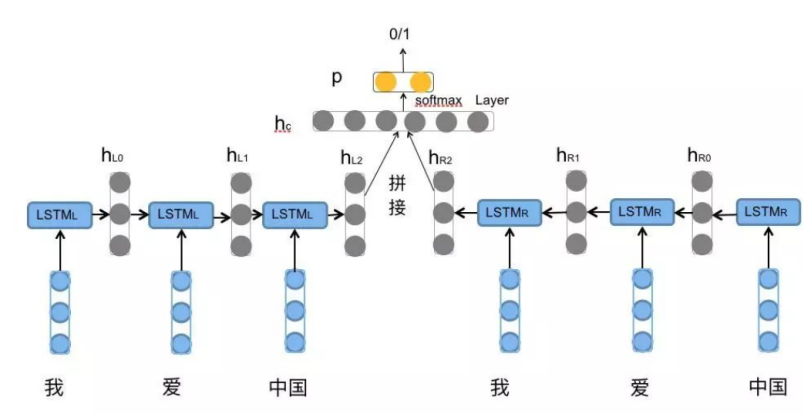
\includegraphics[width=0.8\textwidth]{BiLSTM}
    \caption{BiLSTM结构图}
    \label{fig:bilstm}
\end{figure}

这里主要是用BiLSTM来提取字符级别的特征编码,以及对编码进行序列级别特征提取,得到一个特征融合后的结果,再通过全连接层得到对所有tag的logit,最后使用CRF进行实体的识别预测。

% subsection bilstm (end)

\subsection{CNN+BiLSTM+CRF} % (fold)
\label{sub:cnn}
对于分词任务,当前词的标签基本上只与前几个词有关联。BiLSTM在学习较长句子时,可能因为模型容量问题丢弃一些重要信息,因此在模型中加了一个CNN层,用于提取当前词的局部特征,加入了CNN的模型如下。

\begin{figure}[htbp]
    \centering
    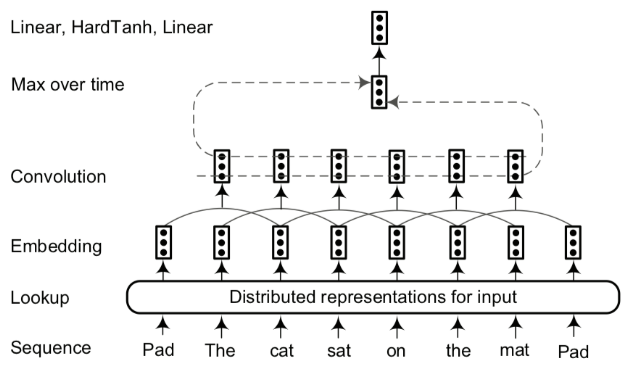
\includegraphics[width=0.6\textwidth]{cnn}
    \caption{基于句法的CNN网络结构}
    \label{fig:encoder}
\end{figure}

句子经过 embedding 层,一个 word 被表示为 N 维度的向量,随后整个句子表示使用卷积编码,进而得到每个 word 的局部特征,卷积层的输出大小与输入的句子长度有关,为了获取固定维度的句子表示,常常使用最大池化操作得到整个句子的全局特征。

% subsection cnn (end)

\subsection{Transformer}
\label{sub:transformer}
项目中使用的BERT和RoBERTa都是基于Transformer的encoder,并且在Transformer的基础上提出了特定的预训练任务,因此在这里对Transformer进行一个系统的介绍,后续的BERT模型和RoBERTa模型则会相对较少的描述,而是更偏重在项目本身的模型结构上。


Transformer是Vaswani等人在《Attention Is All You Need》中提出的,目标是为了提高机器翻译的效率,他们使用了创新的self-attention机制,用于替代RNN循环神经网络,能够高效的并行计算所有位置上的隐藏状态,同时克服了RNN中一直存在的梯度消失问题。Transformer主体分为encoder和decoder,是比较经典的seq2seq模型结构,如图3.3所示,后续的BERT和GPT系列都是只采用了编码器和解码器中的一种,并且都在各类自然语言处理任务中刷新了SOTA。Transformer是实验中的模型BERT和RoBERTa的基础,下面主要对Transformer中的多头自注意力机制、带有位置编码的输入、Layer Normalization、残差连接这几个部分进行简要的介绍。

\begin{figure}[htbp]
    \centering
    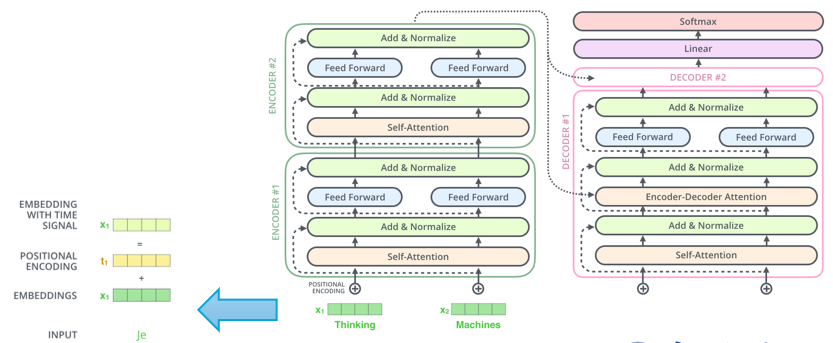
\includegraphics[width=0.9\textwidth]{encoder-decoder}
    \caption{encoder-decoder结构图}
    \label{fig:encoder}
\end{figure}


把encoder和decoder展开后如图\ref{fig:encoder}所示,是由两个encoder和一个decoder的模型结构。可以看到在encoder中主要有positional encoding、self-attention、残差连接、layer Normalization。decoder与encoder的不同主要在于在输入中加入encoder的输出

Transformer中最有名的还是self-attention,它在文本处理中替代了RNN,不用受限于RNN每个时间步对前一个时间步的依赖,以及解决了长距离的梯度消失问题。在自注意力机制被提出之前,已经有了传统的注意力机制,研究者发现文本不同位置的token或者图片中的block都应该有不同的权重,对结果的影响同样有不同的权重。传统的attention机制通常是对隐藏层进行矩阵运算得到,比如对LSTM的hidden state进行dot product或者一些attention变种如hard attention,soft attention,global attention,local attention等。
Self-Attention的实现主要是通过三个矩阵实现,分别是Query矩阵、Keys矩阵、Values矩阵,Query和Key矩阵用于计算权重,Values矩阵代表这个位置token真正的内容,它们分别是通过对输入进行线性变换得到。对于传统attention中的权重energy计算,self-attention使用Query矩阵和Key矩阵进行点乘运算,并经过一个softmax归一化得到。所以从这个角度来说,传统的attention机制也是self-attention的一种特殊情况。得到权重之后便可以用它对Values矩阵进行加权平均,然后得到self-attention层的输出Z矩阵。
Multi-Head Attention其实就是对上面的操作进行多次。会有一组QKV向量。Multi-head是有概率学习到文本的不同语义的。

\begin{figure}[htbp]
    \centering
    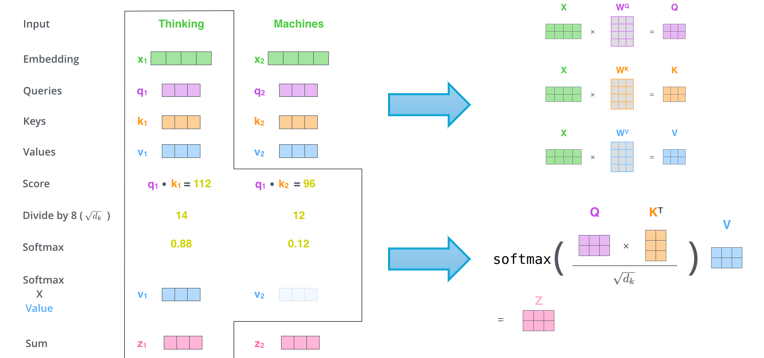
\includegraphics[width=0.9\textwidth]{cal_process}
    \caption{self-attention运算过程}
    \label{fig:encoder}
\end{figure}

Transformer中在进行self-attention之后,会进行残差连接的操作,就是加上之前的输入。
而Layer Normalization其实就是对每个样本的不同特征进行Normalization,之前的BatchNorm,是对所有batch样本的每个特征进行Normalization,Batch Normalization还不可以用于RNN模型,因为同一个节点在不同时刻的分布是明显不同的。
Transformer的残差连接其实是将输入通过self-attention之后,得到输出z1和z2,然后和残差连接的输入x1,x2,加起来,然后经过layer normalization层之后输出给全连接层。全连接层也是有一个残差连接和一个LayerNorm层,最后再输出给上一层。

\begin{figure}[htbp]
    \centering
    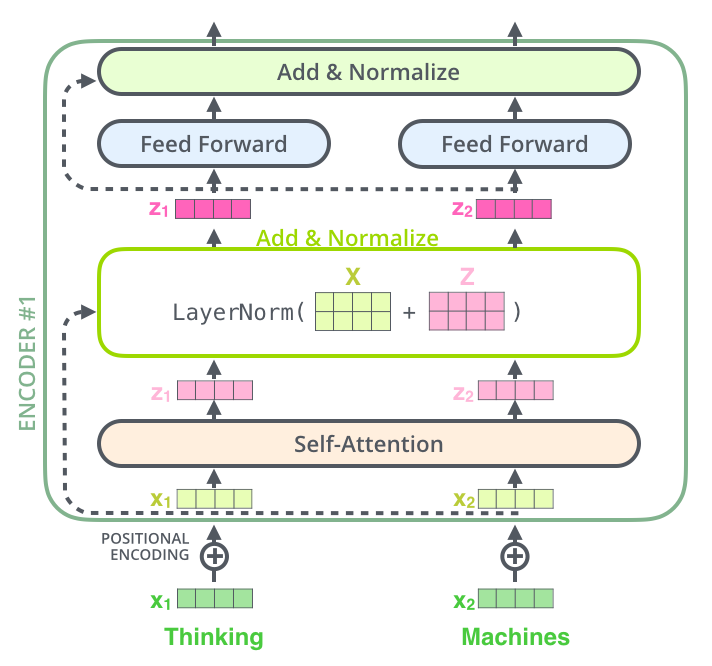
\includegraphics[width=0.45\textwidth]{layer_norm}
    \caption{残差连接和层级归一化过程}
    \label{fig:encoder}
\end{figure}


\subsection{BERT+BiLSTM+CRF} % (fold)
\label{sub:bert}

BERT+BiLSTM+CRF模型中,BERT负责学习输入句子中每个字和符号到对应的实体标签的规律,学得句子中每个字符最大概率的实体标注,过程中考虑每个字符的上下文信息,而CRF负责学习相邻实体标签之间的转移规则,通过引入CRF解决输出的最大分数对应的实体标注依然可能有误的问题。

\begin{figure}[htbp]
    \centering
    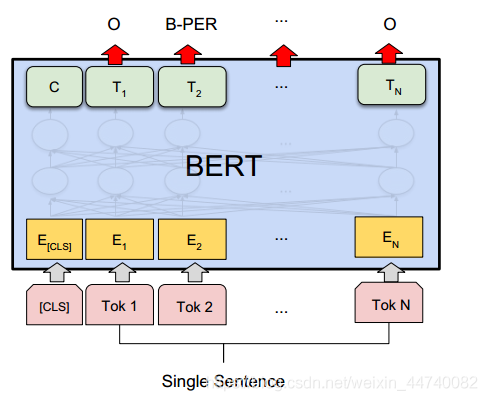
\includegraphics[width=0.45\textwidth]{bert}
    \caption{基于BERT的序列标注结构}
    \label{fig:encoder}
\end{figure}

通过BERT学习序列的状态特征得到一个状态分数,该分数直接输入到CRF层,省去了人工设置状态特征模板的过程。其中,状态分数是根据训练得到的BERT模型的输出计算出来的,转移分数通过CRF层提供的转移分数矩阵计算。


% subsection bert (end)

\subsection{RoBERTA+BiLSTM+CRF} % (fold)
\label{sub:roberta}
RoBERTa是在BERT的一个继承和优化,从模型上来说,RoBERTa基本没有什么太大创新,主要是在BERT基础上做了几点调整:

\begin{enumerate}
    \item 预训练的时间更长,batch size更大,training step减少,实验效果相当或者更好些;
    \item 移除了next predict loss预训练任务,相比于BERT,采用了连续的full-sentences和doc-sentences作为输入(长度最多为512);
    \item 预训练训练的序列更长;
    \item 动态调整Masking机制,即每次输入到序列的Masking都不一样
    \item text encoding,基于bytes的编码可以有效防止unknown问题
    \item 训练数据更多,数据集从16G增加到了160G,训练轮数比BERT有所增加;
    在结果上,RoBERTa超越了BERT和XLNet,这里也选择对它作为BERT的对比实验模型,探究不同预训练任务以及masking策略在对下游情感分析任务上的影响。
\end{enumerate}

命名实体识别预测的过程中,输入方面,使用了RoBERTa为数据集进行编码,由于RoBERTa使用word pieces级别的编码,而实际使用中使用的是词级编码,因此是对每个词进行了word pieces级别的切分,然后对切分的结果使用RoBERTa编码,然后再对每个词的Word pieces进行一个拼接,得到词级别的编码。模型的编码器使用的还是BiLSTM,提取上下文的特征,最后使用全连接层对每个类目进行一个回归,得到对应类目的logit。最后再使用CRF模型限制输出的形式,得到最终的输出结果。

相对于其他模型,甚至BERT模型本身来说,RoBERTa结合CRF强大的地方并不是encoder或者decoder有特殊的处理,而是在输入的embedding阶段,有更强的语义表示,或者说更能代表实体本身的含义。从词级别的拆分来看,也可以用这种方法扩展到实体级别的编码,通过多层级的的编码融合,得到更强的更具有表征意义的输入,对模型的训练是非常有效的。

% subsection roberta (end)

% section model (end)

\section{实验结果分析} % (fold)
\label{sec:analysis}

\subsection{数据集} % (fold)
\label{sub:dataset}
命名实体识别NER任务中,本项目使用来自 CoNLL 2003 共享的的英文数据进行实验,该数据集包含四种不同类型的命名实体:PERSON、LOCATION、ORGANIZATION 和 MISC。 这里使用 BIOUL编码格式,因为之前的研究中相对于默认的BIO编码格式存在显著改进。
% subsection dataset (end)

\subsection{实验结果} % (fold)
\label{sub:res}

本文对所选的传统机器学习模型HMM和CRF,以及以深度学习模型CNN、BiLSTM、BERT、RoBERTa为主的共六个模型的性能进行比较,除传统机器学习模型之外,基于所有这些模型都使用斯坦福大学的 GloVe 词嵌入和相同的超参数运行。



\begin{table}[htbp]
    \begin{center}
    \large 
    \begin{tabular}{lcc}
        \hline
         System & tagging accuracy & F1 scores \\   
        \hline
        
         HMM                &       90.18 & 59.32          \\
         CRF                &       92.00 & 69.36          \\
         BiLSTM+CRF         &       96.89 & 85.15        \\
         CNN+BiLSTM+CRF     &       96.65 & 84.69          \\
         BERT+BiLSTM+CRF    &       97.95 & 90.44         \\
         RoBERTa+BiLSTM+CRF &       98.02 & 91.22      \\
        \hline
    \end{tabular}
    \end{center}
    \caption {对比不同NER模型下的标注准确率和F1得分} 
\end{table}

本文中的模型可以通过 GloVe 嵌入获得 91.22 的最佳 F1 分数。使用了各种机器学习分类器的组合,根据表1结果,BLSTM-CRF模型明显优于 CRF 模型,表明句子特征提取对于命名实体识别任务很重要。BiLSTM+CRF 略微优于 CNN+BiLSTM+CRF,可能是使用了GloVe 不同的词嵌入。然而,BERT+BiLSTM+CRF 明显优于 BiLSTM+CRF,预训练模型BERT的引入大大提高了准确度,而针对BERT模型的改进模型RoBERTa性能也有所提升。
% subsection res (end)

% section analysis (end)

\section{总结}

在对CoNLL2003数据集进行命名实体识别的过程中,我通过阅读相关论文,对命名实体识别的方法有了全局上的了解,并且了解了整个时间线上SOTA的发展变化过程,这让我对命名实体识别这一任务的背景和目标都有了充分的认识。

在传统的实体识别方法上,这里选用了经典的隐马尔科夫模型和条件随机场,它们基于对训练集数据的统计分析完成测试集上面的实体预测。而在深度学习的模型选择上,这里侧重使用基于Transformer的两个预训练模型,分别是BERT和RoBERTa,它们都是通过对大规模语料的预训练,提取出语言本身具有的潜在含义,然后再迁移到命名实体识别这一下游任务中。对比基于CNN和BiLSTM的模型,从准确率和F1分数上也可以看到有很大的提升,这也充分证明了预训练模型的有效性,以及模型的初始化编码对模型能力上的提升作用。


% \bibliographystyle{ACM-Reference-Format}
% \bibliography{ref}

\end{document}